\documentclass{report}

\usepackage{booktabs}
\usepackage{float}


%%%%%%%%%%%%%%%%%%%%%%%%%%%%%%%%%
% PACKAGE IMPORTS
%%%%%%%%%%%%%%%%%%%%%%%%%%%%%%%%%


\usepackage[tmargin=2cm,rmargin=1in,lmargin=1in,margin=0.85in,bmargin=2cm,footskip=.2in]{geometry}
\usepackage{amsmath,amsfonts,amsthm,amssymb,mathtools}
\usepackage[varbb]{newpxmath}
\usepackage{xfrac}
\usepackage[makeroom]{cancel}
\usepackage{mathtools}
\usepackage{bookmark}
\usepackage{enumitem}
\usepackage{hyperref,theoremref}
\hypersetup{
	pdftitle={Assignment},
	colorlinks=true, linkcolor=doc!90,
	bookmarksnumbered=true,
	bookmarksopen=true
}
\usepackage[most,many,breakable]{tcolorbox}
\usepackage{xcolor}
\usepackage{varwidth}
\usepackage{varwidth}
\usepackage{etoolbox}
%\usepackage{authblk}
\usepackage{nameref}
\usepackage{multicol,array}
\usepackage{tikz-cd}
\usepackage[ruled,vlined,linesnumbered]{algorithm2e}
\usepackage{comment} % enables the use of multi-line comments (\ifx \fi) 
\usepackage{import}
\usepackage{xifthen}
\usepackage{pdfpages}
\usepackage{transparent}

\newcommand\mycommfont[1]{\footnotesize\ttfamily\textcolor{blue}{#1}}
\SetCommentSty{mycommfont}
\newcommand{\incfig}[1]{%
    \def\svgwidth{\columnwidth}
    \import{./figures/}{#1.pdf_tex}
}

\usepackage{tikzsymbols}
\renewcommand\qedsymbol{$\Laughey$}


%\usepackage{import}
%\usepackage{xifthen}
%\usepackage{pdfpages}
%\usepackage{transparent}


%%%%%%%%%%%%%%%%%%%%%%%%%%%%%%
% SELF MADE COLORS
%%%%%%%%%%%%%%%%%%%%%%%%%%%%%%



\definecolor{myg}{RGB}{56, 140, 70}
\definecolor{myb}{RGB}{45, 111, 177}
\definecolor{myr}{RGB}{199, 68, 64}
\definecolor{mytheorembg}{HTML}{F2F2F9}
\definecolor{mytheoremfr}{HTML}{00007B}
\definecolor{mylenmabg}{HTML}{FFFAF8}
\definecolor{mylenmafr}{HTML}{983b0f}
\definecolor{mypropbg}{HTML}{f2fbfc}
\definecolor{mypropfr}{HTML}{191971}
\definecolor{myexamplebg}{HTML}{F2FBF8}
\definecolor{myexamplefr}{HTML}{88D6D1}
\definecolor{myexampleti}{HTML}{2A7F7F}
\definecolor{mydefinitbg}{HTML}{E5E5FF}
\definecolor{mydefinitfr}{HTML}{3F3FA3}
\definecolor{notesgreen}{RGB}{0,162,0}
\definecolor{myp}{RGB}{197, 92, 212}
\definecolor{mygr}{HTML}{2C3338}
\definecolor{myred}{RGB}{127,0,0}
\definecolor{myyellow}{RGB}{169,121,69}
\definecolor{myexercisebg}{HTML}{F2FBF8}
\definecolor{myexercisefg}{HTML}{88D6D1}


%%%%%%%%%%%%%%%%%%%%%%%%%%%%
% TCOLORBOX SETUPS
%%%%%%%%%%%%%%%%%%%%%%%%%%%%

\setlength{\parindent}{1cm}
%================================
% THEOREM BOX
%================================

\tcbuselibrary{theorems,skins,hooks}
\newtcbtheorem[number within=section]{Theorem}{Theorem}
{%
	enhanced,
	breakable,
	colback = mytheorembg,
	frame hidden,
	boxrule = 0sp,
	borderline west = {2pt}{0pt}{mytheoremfr},
	sharp corners,
	detach title,
	before upper = \tcbtitle\par\smallskip,
	coltitle = mytheoremfr,
	fonttitle = \bfseries\sffamily,
	description font = \mdseries,
	separator sign none,
	segmentation style={solid, mytheoremfr},
}
{th}

\tcbuselibrary{theorems,skins,hooks}
\newtcbtheorem[number within=chapter]{theorem}{Theorem}
{%
	enhanced,
	breakable,
	colback = mytheorembg,
	frame hidden,
	boxrule = 0sp,
	borderline west = {2pt}{0pt}{mytheoremfr},
	sharp corners,
	detach title,
	before upper = \tcbtitle\par\smallskip,
	coltitle = mytheoremfr,
	fonttitle = \bfseries\sffamily,
	description font = \mdseries,
	separator sign none,
	segmentation style={solid, mytheoremfr},
}
{th}


\tcbuselibrary{theorems,skins,hooks}
\newtcolorbox{Theoremcon}
{%
	enhanced
	,breakable
	,colback = mytheorembg
	,frame hidden
	,boxrule = 0sp
	,borderline west = {2pt}{0pt}{mytheoremfr}
	,sharp corners
	,description font = \mdseries
	,separator sign none
}

%================================
% Corollery
%================================
\tcbuselibrary{theorems,skins,hooks}
\newtcbtheorem[number within=section]{Corollary}{Corollary}
{%
	enhanced
	,breakable
	,colback = myp!10
	,frame hidden
	,boxrule = 0sp
	,borderline west = {2pt}{0pt}{myp!85!black}
	,sharp corners
	,detach title
	,before upper = \tcbtitle\par\smallskip
	,coltitle = myp!85!black
	,fonttitle = \bfseries\sffamily
	,description font = \mdseries
	,separator sign none
	,segmentation style={solid, myp!85!black}
}
{th}
\tcbuselibrary{theorems,skins,hooks}
\newtcbtheorem[number within=chapter]{corollary}{Corollary}
{%
	enhanced
	,breakable
	,colback = myp!10
	,frame hidden
	,boxrule = 0sp
	,borderline west = {2pt}{0pt}{myp!85!black}
	,sharp corners
	,detach title
	,before upper = \tcbtitle\par\smallskip
	,coltitle = myp!85!black
	,fonttitle = \bfseries\sffamily
	,description font = \mdseries
	,separator sign none
	,segmentation style={solid, myp!85!black}
}
{th}


%================================
% LENMA
%================================

\tcbuselibrary{theorems,skins,hooks}
\newtcbtheorem[number within=section]{Lenma}{Lenma}
{%
	enhanced,
	breakable,
	colback = mylenmabg,
	frame hidden,
	boxrule = 0sp,
	borderline west = {2pt}{0pt}{mylenmafr},
	sharp corners,
	detach title,
	before upper = \tcbtitle\par\smallskip,
	coltitle = mylenmafr,
	fonttitle = \bfseries\sffamily,
	description font = \mdseries,
	separator sign none,
	segmentation style={solid, mylenmafr},
}
{th}

\tcbuselibrary{theorems,skins,hooks}
\newtcbtheorem[number within=chapter]{lenma}{Lenma}
{%
	enhanced,
	breakable,
	colback = mylenmabg,
	frame hidden,
	boxrule = 0sp,
	borderline west = {2pt}{0pt}{mylenmafr},
	sharp corners,
	detach title,
	before upper = \tcbtitle\par\smallskip,
	coltitle = mylenmafr,
	fonttitle = \bfseries\sffamily,
	description font = \mdseries,
	separator sign none,
	segmentation style={solid, mylenmafr},
}
{th}


%================================
% PROPOSITION
%================================

\tcbuselibrary{theorems,skins,hooks}
\newtcbtheorem[number within=section]{Prop}{Proposition}
{%
	enhanced,
	breakable,
	colback = mypropbg,
	frame hidden,
	boxrule = 0sp,
	borderline west = {2pt}{0pt}{mypropfr},
	sharp corners,
	detach title,
	before upper = \tcbtitle\par\smallskip,
	coltitle = mypropfr,
	fonttitle = \bfseries\sffamily,
	description font = \mdseries,
	separator sign none,
	segmentation style={solid, mypropfr},
}
{th}

\tcbuselibrary{theorems,skins,hooks}
\newtcbtheorem[number within=chapter]{prop}{Proposition}
{%
	enhanced,
	breakable,
	colback = mypropbg,
	frame hidden,
	boxrule = 0sp,
	borderline west = {2pt}{0pt}{mypropfr},
	sharp corners,
	detach title,
	before upper = \tcbtitle\par\smallskip,
	coltitle = mypropfr,
	fonttitle = \bfseries\sffamily,
	description font = \mdseries,
	separator sign none,
	segmentation style={solid, mypropfr},
}
{th}


%================================
% CLAIM
%================================

\tcbuselibrary{theorems,skins,hooks}
\newtcbtheorem[number within=section]{claim}{Claim}
{%
	enhanced
	,breakable
	,colback = myg!10
	,frame hidden
	,boxrule = 0sp
	,borderline west = {2pt}{0pt}{myg}
	,sharp corners
	,detach title
	,before upper = \tcbtitle\par\smallskip
	,coltitle = myg!85!black
	,fonttitle = \bfseries\sffamily
	,description font = \mdseries
	,separator sign none
	,segmentation style={solid, myg!85!black}
}
{th}



%================================
% Exercise
%================================

\tcbuselibrary{theorems,skins,hooks}
\newtcbtheorem[number within=section]{Exercise}{Exercise}
{%
	enhanced,
	breakable,
	colback = myexercisebg,
	frame hidden,
	boxrule = 0sp,
	borderline west = {2pt}{0pt}{myexercisefg},
	sharp corners,
	detach title,
	before upper = \tcbtitle\par\smallskip,
	coltitle = myexercisefg,
	fonttitle = \bfseries\sffamily,
	description font = \mdseries,
	separator sign none,
	segmentation style={solid, myexercisefg},
}
{th}

\tcbuselibrary{theorems,skins,hooks}
\newtcbtheorem[number within=chapter]{exercise}{Exercise}
{%
	enhanced,
	breakable,
	colback = myexercisebg,
	frame hidden,
	boxrule = 0sp,
	borderline west = {2pt}{0pt}{myexercisefg},
	sharp corners,
	detach title,
	before upper = \tcbtitle\par\smallskip,
	coltitle = myexercisefg,
	fonttitle = \bfseries\sffamily,
	description font = \mdseries,
	separator sign none,
	segmentation style={solid, myexercisefg},
}
{th}

%================================
% EXAMPLE BOX
%================================

\newtcbtheorem[number within=section]{Example}{Example}
{%
	colback = myexamplebg
	,breakable
	,colframe = myexamplefr
	,coltitle = myexampleti
	,boxrule = 1pt
	,sharp corners
	,detach title
	,before upper=\tcbtitle\par\smallskip
	,fonttitle = \bfseries
	,description font = \mdseries
	,separator sign none
	,description delimiters parenthesis
}
{ex}

\newtcbtheorem[number within=chapter]{example}{Example}
{%
	colback = myexamplebg
	,breakable
	,colframe = myexamplefr
	,coltitle = myexampleti
	,boxrule = 1pt
	,sharp corners
	,detach title
	,before upper=\tcbtitle\par\smallskip
	,fonttitle = \bfseries
	,description font = \mdseries
	,separator sign none
	,description delimiters parenthesis
}
{ex}

%================================
% DEFINITION BOX
%================================

\newtcbtheorem[number within=section]{Definition}{Definition}{enhanced,
	before skip=2mm,after skip=2mm, colback=red!5,colframe=red!80!black,boxrule=0.5mm,
	attach boxed title to top left={xshift=1cm,yshift*=1mm-\tcboxedtitleheight}, varwidth boxed title*=-3cm,
	boxed title style={frame code={
					\path[fill=tcbcolback]
					([yshift=-1mm,xshift=-1mm]frame.north west)
					arc[start angle=0,end angle=180,radius=1mm]
					([yshift=-1mm,xshift=1mm]frame.north east)
					arc[start angle=180,end angle=0,radius=1mm];
					\path[left color=tcbcolback!60!black,right color=tcbcolback!60!black,
						middle color=tcbcolback!80!black]
					([xshift=-2mm]frame.north west) -- ([xshift=2mm]frame.north east)
					[rounded corners=1mm]-- ([xshift=1mm,yshift=-1mm]frame.north east)
					-- (frame.south east) -- (frame.south west)
					-- ([xshift=-1mm,yshift=-1mm]frame.north west)
					[sharp corners]-- cycle;
				},interior engine=empty,
		},
	fonttitle=\bfseries,
	title={#2},#1}{def}
\newtcbtheorem[number within=chapter]{definition}{Definition}{enhanced,
	before skip=2mm,after skip=2mm, colback=red!5,colframe=red!80!black,boxrule=0.5mm,
	attach boxed title to top left={xshift=1cm,yshift*=1mm-\tcboxedtitleheight}, varwidth boxed title*=-3cm,
	boxed title style={frame code={
					\path[fill=tcbcolback]
					([yshift=-1mm,xshift=-1mm]frame.north west)
					arc[start angle=0,end angle=180,radius=1mm]
					([yshift=-1mm,xshift=1mm]frame.north east)
					arc[start angle=180,end angle=0,radius=1mm];
					\path[left color=tcbcolback!60!black,right color=tcbcolback!60!black,
						middle color=tcbcolback!80!black]
					([xshift=-2mm]frame.north west) -- ([xshift=2mm]frame.north east)
					[rounded corners=1mm]-- ([xshift=1mm,yshift=-1mm]frame.north east)
					-- (frame.south east) -- (frame.south west)
					-- ([xshift=-1mm,yshift=-1mm]frame.north west)
					[sharp corners]-- cycle;
				},interior engine=empty,
		},
	fonttitle=\bfseries,
	title={#2},#1}{def}



%================================
% Solution BOX
%================================

\makeatletter
\newtcbtheorem{question}{Question}{enhanced,
	breakable,
	colback=white,
	colframe=myb!80!black,
	attach boxed title to top left={yshift*=-\tcboxedtitleheight},
	fonttitle=\bfseries,
	title={#2},
	boxed title size=title,
	boxed title style={%
			sharp corners,
			rounded corners=northwest,
			colback=tcbcolframe,
			boxrule=0pt,
		},
	underlay boxed title={%
			\path[fill=tcbcolframe] (title.south west)--(title.south east)
			to[out=0, in=180] ([xshift=5mm]title.east)--
			(title.center-|frame.east)
			[rounded corners=\kvtcb@arc] |-
			(frame.north) -| cycle;
		},
	#1
}{def}
\makeatother

%================================
% SOLUTION BOX
%================================

\makeatletter
\newtcolorbox{solution}{enhanced,
	breakable,
	colback=white,
	colframe=myg!80!black,
	attach boxed title to top left={yshift*=-\tcboxedtitleheight},
	title=Solution,
	boxed title size=title,
	boxed title style={%
			sharp corners,
			rounded corners=northwest,
			colback=tcbcolframe,
			boxrule=0pt,
		},
	underlay boxed title={%
			\path[fill=tcbcolframe] (title.south west)--(title.south east)
			to[out=0, in=180] ([xshift=5mm]title.east)--
			(title.center-|frame.east)
			[rounded corners=\kvtcb@arc] |-
			(frame.north) -| cycle;
		},
}
\makeatother

%================================
% Question BOX
%================================

\makeatletter
\newtcbtheorem{qstion}{Question}{enhanced,
	breakable,
	colback=white,
	colframe=mygr,
	attach boxed title to top left={yshift*=-\tcboxedtitleheight},
	fonttitle=\bfseries,
	title={#2},
	boxed title size=title,
	boxed title style={%
			sharp corners,
			rounded corners=northwest,
			colback=tcbcolframe,
			boxrule=0pt,
		},
	underlay boxed title={%
			\path[fill=tcbcolframe] (title.south west)--(title.south east)
			to[out=0, in=180] ([xshift=5mm]title.east)--
			(title.center-|frame.east)
			[rounded corners=\kvtcb@arc] |-
			(frame.north) -| cycle;
		},
	#1
}{def}
\makeatother

\newtcbtheorem[number within=chapter]{wconc}{Wrong Concept}{
	breakable,
	enhanced,
	colback=white,
	colframe=myr,
	arc=0pt,
	outer arc=0pt,
	fonttitle=\bfseries\sffamily\large,
	colbacktitle=myr,
	attach boxed title to top left={},
	boxed title style={
			enhanced,
			skin=enhancedfirst jigsaw,
			arc=3pt,
			bottom=0pt,
			interior style={fill=myr}
		},
	#1
}{def}



%================================
% NOTE BOX
%================================

\usetikzlibrary{arrows,calc,shadows.blur}
\tcbuselibrary{skins}
\newtcolorbox{note}[1][]{%
	enhanced jigsaw,
	colback=gray!20!white,%
	colframe=gray!80!black,
	size=small,
	boxrule=1pt,
	title=\textbf{Note:},
	halign title=flush center,
	coltitle=black,
	breakable,
	drop shadow=black!50!white,
	attach boxed title to top left={xshift=1cm,yshift=-\tcboxedtitleheight/2,yshifttext=-\tcboxedtitleheight/2},
	minipage boxed title=1.5cm,
	boxed title style={%
			colback=white,
			size=fbox,
			boxrule=1pt,
			boxsep=2pt,
			underlay={%
					\coordinate (dotA) at ($(interior.west) + (-0.5pt,0)$);
					\coordinate (dotB) at ($(interior.east) + (0.5pt,0)$);
					\begin{scope}
						\clip (interior.north west) rectangle ([xshift=3ex]interior.east);
						\filldraw [white, blur shadow={shadow opacity=60, shadow yshift=-.75ex}, rounded corners=2pt] (interior.north west) rectangle (interior.south east);
					\end{scope}
					\begin{scope}[gray!80!black]
						\fill (dotA) circle (2pt);
						\fill (dotB) circle (2pt);
					\end{scope}
				},
		},
	#1,
}

%%%%%%%%%%%%%%%%%%%%%%%%%%%%%%
% SELF MADE COMMANDS
%%%%%%%%%%%%%%%%%%%%%%%%%%%%%%


\newcommand{\thm}[2]{\begin{Theorem}{#1}{}#2\end{Theorem}}
\newcommand{\cor}[2]{\begin{Corollary}{#1}{}#2\end{Corollary}}
\newcommand{\mlenma}[2]{\begin{Lenma}{#1}{}#2\end{Lenma}}
\newcommand{\mprop}[2]{\begin{Prop}{#1}{}#2\end{Prop}}
\newcommand{\clm}[3]{\begin{claim}{#1}{#2}#3\end{claim}}
\newcommand{\wc}[2]{\begin{wconc}{#1}{}\setlength{\parindent}{1cm}#2\end{wconc}}
\newcommand{\thmcon}[1]{\begin{Theoremcon}{#1}\end{Theoremcon}}
\newcommand{\ex}[2]{\begin{Example}{#1}{}#2\end{Example}}
\newcommand{\dfn}[2]{\begin{Definition}[colbacktitle=red!75!black]{#1}{}#2\end{Definition}}
\newcommand{\dfnc}[2]{\begin{definition}[colbacktitle=red!75!black]{#1}{}#2\end{definition}}
\newcommand{\qs}[2]{\begin{question}{#1}{}#2\end{question}}
\newcommand{\pf}[2]{\begin{myproof}[#1]#2\end{myproof}}
\newcommand{\nt}[1]{\begin{note}#1\end{note}}

\newcommand*\circled[1]{\tikz[baseline=(char.base)]{
		\node[shape=circle,draw,inner sep=1pt] (char) {#1};}}
\newcommand\getcurrentref[1]{%
	\ifnumequal{\value{#1}}{0}
	{??}
	{\the\value{#1}}%
}
\newcommand{\getCurrentSectionNumber}{\getcurrentref{section}}
\newenvironment{myproof}[1][\proofname]{%
	\proof[\bfseries #1: ]%
}{\endproof}

\newcommand{\mclm}[2]{\begin{myclaim}[#1]#2\end{myclaim}}
\newenvironment{myclaim}[1][\claimname]{\proof[\bfseries #1: ]}{}

\newcounter{mylabelcounter}

\makeatletter
\newcommand{\setword}[2]{%
	\phantomsection
	#1\def\@currentlabel{\unexpanded{#1}}\label{#2}%
}
\makeatother




\tikzset{
	symbol/.style={
			draw=none,
			every to/.append style={
					edge node={node [sloped, allow upside down, auto=false]{$#1$}}}
		}
}


% deliminators
\DeclarePairedDelimiter{\abs}{\lvert}{\rvert}
\DeclarePairedDelimiter{\norm}{\lVert}{\rVert}

\DeclarePairedDelimiter{\ceil}{\lceil}{\rceil}
\DeclarePairedDelimiter{\floor}{\lfloor}{\rfloor}
\DeclarePairedDelimiter{\round}{\lfloor}{\rceil}

\newsavebox\diffdbox
\newcommand{\slantedromand}{{\mathpalette\makesl{d}}}
\newcommand{\makesl}[2]{%
\begingroup
\sbox{\diffdbox}{$\mathsurround=0pt#1\mathrm{#2}$}%
\pdfsave
\pdfsetmatrix{1 0 0.2 1}%
\rlap{\usebox{\diffdbox}}%
\pdfrestore
\hskip\wd\diffdbox
\endgroup
}
\newcommand{\dd}[1][]{\ensuremath{\mathop{}\!\ifstrempty{#1}{%
\slantedromand\@ifnextchar^{\hspace{0.2ex}}{\hspace{0.1ex}}}%
{\slantedromand\hspace{0.2ex}^{#1}}}}
\ProvideDocumentCommand\dv{o m g}{%
  \ensuremath{%
    \IfValueTF{#3}{%
      \IfNoValueTF{#1}{%
        \frac{\dd #2}{\dd #3}%
      }{%
        \frac{\dd^{#1} #2}{\dd #3^{#1}}%
      }%
    }{%
      \IfNoValueTF{#1}{%
        \frac{\dd}{\dd #2}%
      }{%
        \frac{\dd^{#1}}{\dd #2^{#1}}%
      }%
    }%
  }%
}
\providecommand*{\pdv}[3][]{\frac{\partial^{#1}#2}{\partial#3^{#1}}}
%  - others
\DeclareMathOperator{\Lap}{\mathcal{L}}
\DeclareMathOperator{\Var}{Var} % varience
\DeclareMathOperator{\Cov}{Cov} % covarience
\DeclareMathOperator{\E}{E} % expected

% Since the amsthm package isn't loaded

% I prefer the slanted \leq
\let\oldleq\leq % save them in case they're every wanted
\let\oldgeq\geq
\renewcommand{\leq}{\leqslant}
\renewcommand{\geq}{\geqslant}

% % redefine matrix env to allow for alignment, use r as default
% \renewcommand*\env@matrix[1][r]{\hskip -\arraycolsep
%     \let\@ifnextchar\new@ifnextchar
%     \array{*\c@MaxMatrixCols #1}}


%\usepackage{framed}
%\usepackage{titletoc}
%\usepackage{etoolbox}
%\usepackage{lmodern}


%\patchcmd{\tableofcontents}{\contentsname}{\sffamily\contentsname}{}{}

%\renewenvironment{leftbar}
%{\def\FrameCommand{\hspace{6em}%
%		{\color{myyellow}\vrule width 2pt depth 6pt}\hspace{1em}}%
%	\MakeFramed{\parshape 1 0cm \dimexpr\textwidth-6em\relax\FrameRestore}\vskip2pt%
%}
%{\endMakeFramed}

%\titlecontents{chapter}
%[0em]{\vspace*{2\baselineskip}}
%{\parbox{4.5em}{%
%		\hfill\Huge\sffamily\bfseries\color{myred}\thecontentspage}%
%	\vspace*{-2.3\baselineskip}\leftbar\textsc{\small\chaptername~\thecontentslabel}\\\sffamily}
%{}{\endleftbar}
%\titlecontents{section}
%[8.4em]
%{\sffamily\contentslabel{3em}}{}{}
%{\hspace{0.5em}\nobreak\itshape\color{myred}\contentspage}
%\titlecontents{subsection}
%[8.4em]
%{\sffamily\contentslabel{3em}}{}{}  
%{\hspace{0.5em}\nobreak\itshape\color{myred}\contentspage}



%%%%%%%%%%%%%%%%%%%%%%%%%%%%%%%%%%%%%%%%%%%
% TABLE OF CONTENTS
%%%%%%%%%%%%%%%%%%%%%%%%%%%%%%%%%%%%%%%%%%%

\usepackage{tikz}
\definecolor{doc}{RGB}{0,60,110}
\usepackage{titletoc}
\contentsmargin{0cm}
\titlecontents{chapter}[3.7pc]
{\addvspace{30pt}%
	\begin{tikzpicture}[remember picture, overlay]%
		\draw[fill=doc!60,draw=doc!60] (-7,-.1) rectangle (-0.9,.5);%
		\pgftext[left,x=-3.5cm,y=0.2cm]{\color{white}\Large\sc\bfseries Chapter\ \thecontentslabel};%
	\end{tikzpicture}\color{doc!60}\large\sc\bfseries}%
{}
{}
{\;\titlerule\;\large\sc\bfseries Page \thecontentspage
	\begin{tikzpicture}[remember picture, overlay]
		\draw[fill=doc!60,draw=doc!60] (2pt,0) rectangle (4,0.1pt);
	\end{tikzpicture}}%
\titlecontents{section}[3.7pc]
{\addvspace{2pt}}
{\contentslabel[\thecontentslabel]{2pc}}
{}
{\hfill\small \thecontentspage}
[]
\titlecontents*{subsection}[3.7pc]
{\addvspace{-1pt}\small}
{}
{}
{\ --- \small\thecontentspage}
[ \textbullet\ ][]

\makeatletter
\renewcommand{\tableofcontents}{%
	\chapter*{%
	  \vspace*{-20\p@}%
	  \begin{tikzpicture}[remember picture, overlay]%
		  \pgftext[right,x=15cm,y=0.2cm]{\color{doc!60}\Huge\sc\bfseries \contentsname};%
		  \draw[fill=doc!60,draw=doc!60] (13,-.75) rectangle (20,1);%
		  \clip (13,-.75) rectangle (20,1);
		  \pgftext[right,x=15cm,y=0.2cm]{\color{white}\Huge\sc\bfseries \contentsname};%
	  \end{tikzpicture}}%
	\@starttoc{toc}}
\makeatother


% My commands %
\newcommand{\innerproduct}[2]{\langle #1, #2 \rangle}
\newcommand{\generators}[1]{\langle #1 \rangle}

%From M275 "Topology" at SJSU
\newcommand{\id}{\mathrm{id}}
\newcommand{\taking}[1]{\xrightarrow{#1}}
\newcommand{\inv}{^{-1}}

%From M170 "Introduction to Graph Theory" at SJSU
\DeclareMathOperator{\diam}{diam}
\DeclareMathOperator{\ord}{ord}
\newcommand{\defeq}{\overset{\mathrm{def}}{=}}

%From the USAMO .tex files
\newcommand{\ts}{\textsuperscript}
\newcommand{\dg}{^\circ}
\newcommand{\ii}{\item}

% % From Math 55 and Math 145 at Harvard
% \newenvironment{subproof}[1][Proof]{%
% \begin{proof}[#1] \renewcommand{\qedsymbol}{$\blacksquare$}}%
% {\end{proof}}

\newcommand{\liff}{\leftrightarrow}
\newcommand{\lthen}{\rightarrow}
\newcommand{\opname}{\operatorname}
\newcommand{\surjto}{\twoheadrightarrow}
\newcommand{\injto}{\hookrightarrow}
\newcommand{\On}{\mathrm{On}} % ordinals
\DeclareMathOperator{\img}{im} % Image
\DeclareMathOperator{\Img}{Im} % Image
\DeclareMathOperator{\coker}{coker} % Cokernel
\DeclareMathOperator{\Coker}{Coker} % Cokernel
\DeclareMathOperator{\Ker}{Ker} % Kernel
\DeclareMathOperator{\rank}{rank}
\DeclareMathOperator{\Spec}{Spec} % spectrum
\DeclareMathOperator{\Tr}{Tr} % trace
\DeclareMathOperator{\pr}{pr} % projection
\DeclareMathOperator{\ext}{ext} % extension
\DeclareMathOperator{\pred}{pred} % predecessor
\DeclareMathOperator{\dom}{dom} % domain
\DeclareMathOperator{\ran}{ran} % range
\DeclareMathOperator{\Hom}{Hom} % homomorphism
\DeclareMathOperator{\Mor}{Mor} % morphisms
\DeclareMathOperator{\End}{End} % endomorphism

\newcommand{\eps}{\epsilon}
\newcommand{\veps}{\varepsilon}
\newcommand{\ol}{\overline}
\newcommand{\ul}{\underline}
\newcommand{\wt}{\widetilde}
\newcommand{\wh}{\widehat}
\newcommand{\vocab}[1]{\textbf{\color{blue} #1}}
\providecommand{\half}{\frac{1}{2}}
\newcommand{\dang}{\measuredangle} %% Directed angle
\newcommand{\ray}[1]{\overrightarrow{#1}}
\newcommand{\seg}[1]{\overline{#1}}
\newcommand{\arc}[1]{\wideparen{#1}}
\DeclareMathOperator{\cis}{cis}
\DeclareMathOperator*{\lcm}{lcm}
\DeclareMathOperator*{\argmin}{arg min}
\DeclareMathOperator*{\argmax}{arg max}
\newcommand{\cycsum}{\sum_{\mathrm{cyc}}}
\newcommand{\symsum}{\sum_{\mathrm{sym}}}
\newcommand{\cycprod}{\prod_{\mathrm{cyc}}}
\newcommand{\symprod}{\prod_{\mathrm{sym}}}
\newcommand{\Qed}{\begin{flushright}\qed\end{flushright}}
\newcommand{\parinn}{\setlength{\parindent}{1cm}}
\newcommand{\parinf}{\setlength{\parindent}{0cm}}
% \newcommand{\norm}{\|\cdot\|}
\newcommand{\inorm}{\norm_{\infty}}
\newcommand{\opensets}{\{V_{\alpha}\}_{\alpha\in I}}
\newcommand{\oset}{V_{\alpha}}
\newcommand{\opset}[1]{V_{\alpha_{#1}}}
\newcommand{\lub}{\text{lub}}
\newcommand{\del}[2]{\frac{\partial #1}{\partial #2}}
\newcommand{\Del}[3]{\frac{\partial^{#1} #2}{\partial^{#1} #3}}
\newcommand{\deld}[2]{\dfrac{\partial #1}{\partial #2}}
\newcommand{\Deld}[3]{\dfrac{\partial^{#1} #2}{\partial^{#1} #3}}
\newcommand{\lm}{\lambda}
\newcommand{\uin}{\mathbin{\rotatebox[origin=c]{90}{$\in$}}}
\newcommand{\usubset}{\mathbin{\rotatebox[origin=c]{90}{$\subset$}}}
\newcommand{\lt}{\left}
\newcommand{\rt}{\right}
\newcommand{\bs}[1]{\boldsymbol{#1}}
\newcommand{\exs}{\exists}
\newcommand{\st}{\strut}
\newcommand{\dps}[1]{\displaystyle{#1}}

\newcommand{\sol}{\setlength{\parindent}{0cm}\textbf{\textit{Solution:}}\setlength{\parindent}{1cm} }
\newcommand{\solve}[1]{\setlength{\parindent}{0cm}\textbf{\textit{Solution: }}\setlength{\parindent}{1cm}#1 \Qed}

% Things Lie
\newcommand{\kb}{\mathfrak b}
\newcommand{\kg}{\mathfrak g}
\newcommand{\kh}{\mathfrak h}
\newcommand{\kn}{\mathfrak n}
\newcommand{\ku}{\mathfrak u}
\newcommand{\kz}{\mathfrak z}
\DeclareMathOperator{\Ext}{Ext} % Ext functor
\DeclareMathOperator{\Tor}{Tor} % Tor functor
\newcommand{\gl}{\opname{\mathfrak{gl}}} % frak gl group
\renewcommand{\sl}{\opname{\mathfrak{sl}}} % frak sl group chktex 6

% More script letters etc.
\newcommand{\SA}{\mathcal A}
\newcommand{\SB}{\mathcal B}
\newcommand{\SC}{\mathcal C}
\newcommand{\SF}{\mathcal F}
\newcommand{\SG}{\mathcal G}
\newcommand{\SH}{\mathcal H}
\newcommand{\OO}{\mathcal O}

\newcommand{\SCA}{\mathscr A}
\newcommand{\SCB}{\mathscr B}
\newcommand{\SCC}{\mathscr C}
\newcommand{\SCD}{\mathscr D}
\newcommand{\SCE}{\mathscr E}
\newcommand{\SCF}{\mathscr F}
\newcommand{\SCG}{\mathscr G}
\newcommand{\SCH}{\mathscr H}

% Mathfrak primes
\newcommand{\km}{\mathfrak m}
\newcommand{\kp}{\mathfrak p}
\newcommand{\kq}{\mathfrak q}

% number sets
\newcommand{\RR}[1][]{\ensuremath{\ifstrempty{#1}{\mathbb{R}}{\mathbb{R}^{#1}}}}
\newcommand{\NN}[1][]{\ensuremath{\ifstrempty{#1}{\mathbb{N}}{\mathbb{N}^{#1}}}}
\newcommand{\ZZ}[1][]{\ensuremath{\ifstrempty{#1}{\mathbb{Z}}{\mathbb{Z}^{#1}}}}
\newcommand{\QQ}[1][]{\ensuremath{\ifstrempty{#1}{\mathbb{Q}}{\mathbb{Q}^{#1}}}}
\newcommand{\CC}[1][]{\ensuremath{\ifstrempty{#1}{\mathbb{C}}{\mathbb{C}^{#1}}}}
\newcommand{\PP}[1][]{\ensuremath{\ifstrempty{#1}{\mathbb{P}}{\mathbb{P}^{#1}}}}
\newcommand{\HH}[1][]{\ensuremath{\ifstrempty{#1}{\mathbb{H}}{\mathbb{H}^{#1}}}}
\newcommand{\FF}[1][]{\ensuremath{\ifstrempty{#1}{\mathbb{F}}{\mathbb{F}^{#1}}}}
% expected value
\newcommand{\EE}{\ensuremath{\mathbb{E}}}
\newcommand{\charin}{\text{ char }}
\DeclareMathOperator{\sign}{sign}
\DeclareMathOperator{\Aut}{Aut}
\DeclareMathOperator{\Inn}{Inn}
\DeclareMathOperator{\Syl}{Syl}
\DeclareMathOperator{\Gal}{Gal}
\DeclareMathOperator{\GL}{GL} % General linear group
\DeclareMathOperator{\SL}{SL} % Special linear group

%---------------------------------------
% BlackBoard Math Fonts :-
%---------------------------------------

%Captital Letters
\newcommand{\bbA}{\mathbb{A}}	\newcommand{\bbB}{\mathbb{B}}
\newcommand{\bbC}{\mathbb{C}}	\newcommand{\bbD}{\mathbb{D}}
\newcommand{\bbE}{\mathbb{E}}	\newcommand{\bbF}{\mathbb{F}}
\newcommand{\bbG}{\mathbb{G}}	\newcommand{\bbH}{\mathbb{H}}
\newcommand{\bbI}{\mathbb{I}}	\newcommand{\bbJ}{\mathbb{J}}
\newcommand{\bbK}{\mathbb{K}}	\newcommand{\bbL}{\mathbb{L}}
\newcommand{\bbM}{\mathbb{M}}	\newcommand{\bbN}{\mathbb{N}}
\newcommand{\bbO}{\mathbb{O}}	\newcommand{\bbP}{\mathbb{P}}
\newcommand{\bbQ}{\mathbb{Q}}	\newcommand{\bbR}{\mathbb{R}}
\newcommand{\bbS}{\mathbb{S}}	\newcommand{\bbT}{\mathbb{T}}
\newcommand{\bbU}{\mathbb{U}}	\newcommand{\bbV}{\mathbb{V}}
\newcommand{\bbW}{\mathbb{W}}	\newcommand{\bbX}{\mathbb{X}}
\newcommand{\bbY}{\mathbb{Y}}	\newcommand{\bbZ}{\mathbb{Z}}

%---------------------------------------
% MathCal Fonts :-
%---------------------------------------

%Captital Letters
\newcommand{\mcA}{\mathcal{A}}	\newcommand{\mcB}{\mathcal{B}}
\newcommand{\mcC}{\mathcal{C}}	\newcommand{\mcD}{\mathcal{D}}
\newcommand{\mcE}{\mathcal{E}}	\newcommand{\mcF}{\mathcal{F}}
\newcommand{\mcG}{\mathcal{G}}	\newcommand{\mcH}{\mathcal{H}}
\newcommand{\mcI}{\mathcal{I}}	\newcommand{\mcJ}{\mathcal{J}}
\newcommand{\mcK}{\mathcal{K}}	\newcommand{\mcL}{\mathcal{L}}
\newcommand{\mcM}{\mathcal{M}}	\newcommand{\mcN}{\mathcal{N}}
\newcommand{\mcO}{\mathcal{O}}	\newcommand{\mcP}{\mathcal{P}}
\newcommand{\mcQ}{\mathcal{Q}}	\newcommand{\mcR}{\mathcal{R}}
\newcommand{\mcS}{\mathcal{S}}	\newcommand{\mcT}{\mathcal{T}}
\newcommand{\mcU}{\mathcal{U}}	\newcommand{\mcV}{\mathcal{V}}
\newcommand{\mcW}{\mathcal{W}}	\newcommand{\mcX}{\mathcal{X}}
\newcommand{\mcY}{\mathcal{Y}}	\newcommand{\mcZ}{\mathcal{Z}}


%---------------------------------------
% Bold Math Fonts :-
%---------------------------------------

%Captital Letters
\newcommand{\bmA}{\boldsymbol{A}}	\newcommand{\bmB}{\boldsymbol{B}}
\newcommand{\bmC}{\boldsymbol{C}}	\newcommand{\bmD}{\boldsymbol{D}}
\newcommand{\bmE}{\boldsymbol{E}}	\newcommand{\bmF}{\boldsymbol{F}}
\newcommand{\bmG}{\boldsymbol{G}}	\newcommand{\bmH}{\boldsymbol{H}}
\newcommand{\bmI}{\boldsymbol{I}}	\newcommand{\bmJ}{\boldsymbol{J}}
\newcommand{\bmK}{\boldsymbol{K}}	\newcommand{\bmL}{\boldsymbol{L}}
\newcommand{\bmM}{\boldsymbol{M}}	\newcommand{\bmN}{\boldsymbol{N}}
\newcommand{\bmO}{\boldsymbol{O}}	\newcommand{\bmP}{\boldsymbol{P}}
\newcommand{\bmQ}{\boldsymbol{Q}}	\newcommand{\bmR}{\boldsymbol{R}}
\newcommand{\bmS}{\boldsymbol{S}}	\newcommand{\bmT}{\boldsymbol{T}}
\newcommand{\bmU}{\boldsymbol{U}}	\newcommand{\bmV}{\boldsymbol{V}}
\newcommand{\bmW}{\boldsymbol{W}}	\newcommand{\bmX}{\boldsymbol{X}}
\newcommand{\bmY}{\boldsymbol{Y}}	\newcommand{\bmZ}{\boldsymbol{Z}}
%Small Letters
\newcommand{\bma}{\boldsymbol{a}}	\newcommand{\bmb}{\boldsymbol{b}}
\newcommand{\bmc}{\boldsymbol{c}}	\newcommand{\bmd}{\boldsymbol{d}}
\newcommand{\bme}{\boldsymbol{e}}	\newcommand{\bmf}{\boldsymbol{f}}
\newcommand{\bmg}{\boldsymbol{g}}	\newcommand{\bmh}{\boldsymbol{h}}
\newcommand{\bmi}{\boldsymbol{i}}	\newcommand{\bmj}{\boldsymbol{j}}
\newcommand{\bmk}{\boldsymbol{k}}	\newcommand{\bml}{\boldsymbol{l}}
\newcommand{\bmm}{\boldsymbol{m}}	\newcommand{\bmn}{\boldsymbol{n}}
\newcommand{\bmo}{\boldsymbol{o}}	\newcommand{\bmp}{\boldsymbol{p}}
\newcommand{\bmq}{\boldsymbol{q}}	\newcommand{\bmr}{\boldsymbol{r}}
\newcommand{\bms}{\boldsymbol{s}}	\newcommand{\bmt}{\boldsymbol{t}}
\newcommand{\bmu}{\boldsymbol{u}}	\newcommand{\bmv}{\boldsymbol{v}}
\newcommand{\bmw}{\boldsymbol{w}}	\newcommand{\bmx}{\boldsymbol{x}}
\newcommand{\bmy}{\boldsymbol{y}}	\newcommand{\bmz}{\boldsymbol{z}}

%---------------------------------------
% Scr Math Fonts :-
%---------------------------------------

\newcommand{\sA}{{\mathscr{A}}}   \newcommand{\sB}{{\mathscr{B}}}
\newcommand{\sC}{{\mathscr{C}}}   \newcommand{\sD}{{\mathscr{D}}}
\newcommand{\sE}{{\mathscr{E}}}   \newcommand{\sF}{{\mathscr{F}}}
\newcommand{\sG}{{\mathscr{G}}}   \newcommand{\sH}{{\mathscr{H}}}
\newcommand{\sI}{{\mathscr{I}}}   \newcommand{\sJ}{{\mathscr{J}}}
\newcommand{\sK}{{\mathscr{K}}}   \newcommand{\sL}{{\mathscr{L}}}
\newcommand{\sM}{{\mathscr{M}}}   \newcommand{\sN}{{\mathscr{N}}}
\newcommand{\sO}{{\mathscr{O}}}   \newcommand{\sP}{{\mathscr{P}}}
\newcommand{\sQ}{{\mathscr{Q}}}   \newcommand{\sR}{{\mathscr{R}}}
\newcommand{\sS}{{\mathscr{S}}}   \newcommand{\sT}{{\mathscr{T}}}
\newcommand{\sU}{{\mathscr{U}}}   \newcommand{\sV}{{\mathscr{V}}}
\newcommand{\sW}{{\mathscr{W}}}   \newcommand{\sX}{{\mathscr{X}}}
\newcommand{\sY}{{\mathscr{Y}}}   \newcommand{\sZ}{{\mathscr{Z}}}


%---------------------------------------
% Math Fraktur Font
%---------------------------------------

%Captital Letters
\newcommand{\mfA}{\mathfrak{A}}	\newcommand{\mfB}{\mathfrak{B}}
\newcommand{\mfC}{\mathfrak{C}}	\newcommand{\mfD}{\mathfrak{D}}
\newcommand{\mfE}{\mathfrak{E}}	\newcommand{\mfF}{\mathfrak{F}}
\newcommand{\mfG}{\mathfrak{G}}	\newcommand{\mfH}{\mathfrak{H}}
\newcommand{\mfI}{\mathfrak{I}}	\newcommand{\mfJ}{\mathfrak{J}}
\newcommand{\mfK}{\mathfrak{K}}	\newcommand{\mfL}{\mathfrak{L}}
\newcommand{\mfM}{\mathfrak{M}}	\newcommand{\mfN}{\mathfrak{N}}
\newcommand{\mfO}{\mathfrak{O}}	\newcommand{\mfP}{\mathfrak{P}}
\newcommand{\mfQ}{\mathfrak{Q}}	\newcommand{\mfR}{\mathfrak{R}}
\newcommand{\mfS}{\mathfrak{S}}	\newcommand{\mfT}{\mathfrak{T}}
\newcommand{\mfU}{\mathfrak{U}}	\newcommand{\mfV}{\mathfrak{V}}
\newcommand{\mfW}{\mathfrak{W}}	\newcommand{\mfX}{\mathfrak{X}}
\newcommand{\mfY}{\mathfrak{Y}}	\newcommand{\mfZ}{\mathfrak{Z}}
%Small Letters
\newcommand{\mfa}{\mathfrak{a}}	\newcommand{\mfb}{\mathfrak{b}}
\newcommand{\mfc}{\mathfrak{c}}	\newcommand{\mfd}{\mathfrak{d}}
\newcommand{\mfe}{\mathfrak{e}}	\newcommand{\mff}{\mathfrak{f}}
\newcommand{\mfg}{\mathfrak{g}}	\newcommand{\mfh}{\mathfrak{h}}
\newcommand{\mfi}{\mathfrak{i}}	\newcommand{\mfj}{\mathfrak{j}}
\newcommand{\mfk}{\mathfrak{k}}	\newcommand{\mfl}{\mathfrak{l}}
\newcommand{\mfm}{\mathfrak{m}}	\newcommand{\mfn}{\mathfrak{n}}
\newcommand{\mfo}{\mathfrak{o}}	\newcommand{\mfp}{\mathfrak{p}}
\newcommand{\mfq}{\mathfrak{q}}	\newcommand{\mfr}{\mathfrak{r}}
\newcommand{\mfs}{\mathfrak{s}}	\newcommand{\mft}{\mathfrak{t}}
\newcommand{\mfu}{\mathfrak{u}}	\newcommand{\mfv}{\mathfrak{v}}
\newcommand{\mfw}{\mathfrak{w}}	\newcommand{\mfx}{\mathfrak{x}}
\newcommand{\mfy}{\mathfrak{y}}	\newcommand{\mfz}{\mathfrak{z}}


\newcommand{\D}{\mathcal{D}}
\newcommand{\et}[1]{%
    \mathrm{error}_{\text{train}(#1)}%
}

\newcommand{\ed}[1]{%
    \mathrm{error}_{\mathcal{D}(#1)}%
}
\newcommand{\vectdef}[1]{
    \textbf{#1} = (#1_1,#1_2,\dots, #1_n )
}


% voglio fare un titolo
\graphicspath{{paginette/imgs}}

\begin{document}

\tableofcontents

\chapter{Decision Trees}

Let's start with training set:
\dfn{
Training set
}{
    is defined training set a \textit{set of examples}, where:
    \begin{math}
        \langle x^{(i)}, y^{(i)} \rangle
    \end{math}
    where:
    \begin{itemize}
        \item \textit{i} is the instance of the example 
        \item $x^{(i)}\in X$ is the set of \textit{input} 
        \item $y^{(i)}\in Y$ is the set of \textit{output}
    \end{itemize}
}

the problem of machine learning is to find a function $h:X\to Y$ that approximates the real function $f:X\to Y$. We have two types of problems:
\begin{itemize}
    \item \textbf{Classification}: $Y$ is a discrete set of values (e.g. $\{0,1\}$)
    \item \textbf{Regression}: $Y$ is a continuous set of values (e.g. $\mathbb{R}$)
\end{itemize}
\section{Hypothesis space}

In machine learning the \textit{hypothesis space} $H$ is defined as the set of all possible functions that can be used to approximate the real function $f:X\to Y$. Formally:
\dfn{
Hypothesis space
}{
    A hypothesis space $H$ is defined as the set:
    \begin{math}
        H = \{h | h:X\to Y\}
    \end{math}
    where:
    \begin{itemize}
        \item $h$ is a function (hypothesis) that maps input $X$ to output $Y$
        \item $X$ the input space (features, domain of data).
        \item $Y$ the output space (labels, range of data).
        \item $|H|$ is the size of the hypothesis space (number of possible hypotheses)
    \end{itemize}
}
this let us to define the model:
\dfn{
Model
}{
    A model is a way to compute a function $h\in H$ from the training set.
}

\ex{
    Decision tree
}{
    A good day to play tennis? Our function $F$ is:
    \[
        \mathbb{F}:Outlook \times Humidity \times Wind \times Temp \to Play Tennis?
    \] 
    \begin{center}
        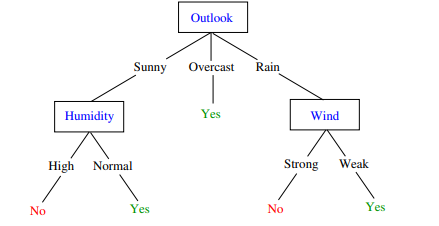
\includegraphics[width=0.6\textwidth]{dtree.png}
    \end{center}
    where:
    \begin{itemize}
        \item $Outlook\in\{Sunny, Overcast, Rain\}$
        \item $Humidity\in\{High, Normal\}$
        \item $Wind\in\{Weak, Strong\}$
        \item $PlayTennis?\in\{Yes, No\}$
    \end{itemize}

    Every node tests an attribute. Each branch corresponds to one of the possible values for that attribute. Each leaf node assigns a classification (Yes or No), in other words predicts the answer $Y$.

    The prblem configurationg is the following:
    \begin{itemize}
        \item $X$ is the set of all possible $x\in X$ that corresponds to a vector of attributes $(Outlook, Humidity, Wind, Temp)$ 
        \item Target function $f:X\to Y$ is the function that maps the attributes to the target variable $PlayTennis?$ (booleans)
        \item Hypothesis space $H=\{h | h:X\to Y\}$ is the set of all possible decision trees that can be constructed using the attributes in $X$ to predict the target variable $Y$
    \end{itemize}

    \begin{center}
        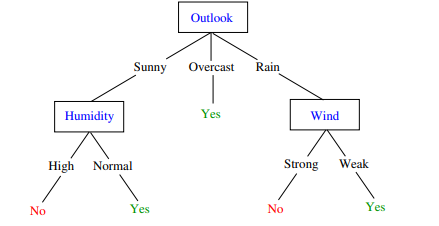
\includegraphics[width=0.6\textwidth]{dtree.png}
    \end{center}
}

\subsection{Top-down inductive construction}
Let $X = X_1 \times X_2 \dots \times X_n $ where $X_i = \{\text{Truee},\text{False}\}$


Can we represent, for instance, $ Y = X_2 \land X_5$? or $Y=X_2 \land X_5 \lor (\lnot X_3) \land X_4 \land X_1 ? $

and:

\begin{itemize}
    \item do we have a decision tree for each h in the space hypothesis?
    \item if the tree exists, is it unique?
    \item if it is not unique, do we have a preference?
\end{itemize}

\thm{
    Basta - Bonzo
}{
    Main loop:
    \begin{itemize}
        \item \textbf{Pick the "best" attribute $X_i$}: At the current node, choose which featue/attribute will bwst split the training data.
        
        Best means: the attribute that gives the most information gain
        \item \textbf{Create a child node for each possible value of $X_i$}: for instance if attribute is "weather" with values "sunny", "rainy", "overcast", create three child nodes.
        \item \textbf{check if all examples in the chils node are pure}: if all examples belong to the same class (e.g., all "yes" or all "no"), make that node a leaf node with that class label. If not repeat the process recursively for each child node.
    \end{itemize}
}

\subsection{Entropy}

\dfn{
    Entropy
}{
    The entropy $H(S)$ of a set of examples $S$ is defined as:
    \[
        H(S) = -\sum_{i=1}^{n} P(X=i)\log_2 P(X=i)
    \]
    where:
    \begin{itemize}
        \item $P(X=i)$ is the proportion of examples in $S$ that belong to class $i$
        \item $n$ is the number of classes (the number of possibile values of $X$)
    \end{itemize}
}

In other words, Entropy meausers the \textit{degree of uncertainty} of the information. It is maximal when $X$ is uniformly distributed (all classes have the same probability) and minimal (zero) when all examples belong to the same class (pure set)
\begin{center}
    \IfFileExists{imgs/entropy.png}{%
        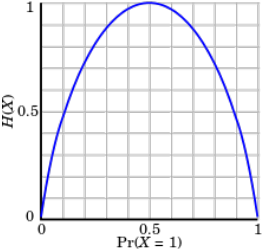
\includegraphics[width=0.6\textwidth]{imgs/entropy.png}%
    }{%
        \fbox{\parbox{0.6\textwidth}{\centering Missing image: imgs/entropy.png}}%
    }
\end{center}

\subsubsection{Information Theory (Shannon 1948)}
The entropy is the average amount of information produced by a stochastic source of data. The \textit{information} is associated to the \textit{probability} of each datum (the surprise element):
\begin{itemize}
    \item An event with probability 1 (certain event) provides no information (no surprise): \(I(1)=0\).
    \item An event with probability 0 (impossible event) provides infinite information (really surprising): \(I(0)=\infty\).
    \item Given two independent events \(A\) and \(B\), the information provided by both events is the sum of the information provided by each event:
    \[
        I(A \cap B) = I(A) + I(B)
    \]
\end{itemize}
So is natoral defining 
\[
    I(p) = -\log_2(p)
\]
\subsubsection{Code Theory (Shannon-Fano 1949, Huffman 1952)}
The entropy is also related to the avarage number of bits required to transmit outcomes produces by a stochastic source process $x$.

Let suppose to have $n$ events with same probability \(p_i = \frac{1}{n}\). Home many bits do we need to encode these events? The answer is \(\log_2(n)\) bits. For instance, if we have 4 events, we need 2 bits to encode them:.

In this case:
\[
    H(X) = -\sum_{i=1}^{n} P(X=i)\log_2 P(X=i) = - \sum_{i=1}^{n} \frac{1}{n} \log_2 \frac{1}{n} = \log_2(n)
\]

\subsection{Information Gain}

In a decision tree, the goal is to maximize the information gain during the execution of the algorithm. 
In other words, the final split should result in the minimum possible impurity. 
Here are the main formulas:

\thm{Entropy of $X$}{
    \[
        H(X) = -\sum_{i=1}^{n} P(X=i)\log_2 P(X=i)
    \]
}

\thm{Conditional Entropy of $X$ given a specific $Y=v$}{
    \label{thm:cexyv}
    \[
        H(X \mid Y=v) = -\sum_{i=1}^{n} P(X=i \mid Y=v)\log_2 P(X=i \mid Y=v)
    \]
}

This measures the entropy of $X$ restricted to the subgroup where $Y=v$.

\thm{Conditional Entropy of $X$ given $Y$}{
    \[
        H(X \mid Y) = \sum_{v=1}^{m} P(Y=v) \, H(X \mid Y=v)
    \]
}

This is the generalization of \ref{thm:cexyv}, used to evaluate the utility of an attribute. 
It measures the average impurity that remains in $X$ after splitting the data using all possible values of $Y$.

\thm{
    Information Gain between $X$ and $Y$
}{
    Here we are!
    \begin{math}
        I(X, Y ) = H(X) - H(X\|Y ) = H(Y ) - H(Y \|X)
    \end{math}
}

\ex{Information gain}{
    Let us measure the entropy reduction of the target variable $Y$ due to some attribute $X$, that is the information gain $I(Y , X)$ between $Y$ and $X$

    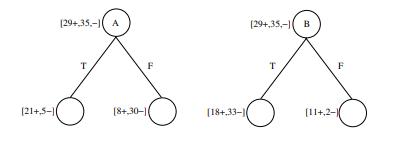
\includegraphics{ig.png}

    \[
    \begin{aligned}
    H(Y) &= -\frac{29}{64}\log_2\!\left(\tfrac{29}{64}\right) - \frac{35}{64}\log_2\!\left(\tfrac{35}{64}\right) = 0.994 \\[6pt]
    H(Y \mid A=T) &= -\frac{21}{26}\log_2\!\left(\tfrac{21}{26}\right) - \frac{5}{26}\log_2\!\left(\tfrac{5}{26}\right) = 0.706 \\[6pt]
    H(Y \mid A=F) &= -\frac{8}{38}\log_2\!\left(\tfrac{8}{38}\right) - \frac{30}{38}\log_2\!\left(\tfrac{30}{38}\right) = 0.742 \\[6pt]
    H(Y \mid A) &= 0.706 \cdot \tfrac{26}{64} \;+\; 0.742 \cdot \tfrac{38}{64} = 0.726 \\[6pt]
    I(Y, A) &= H(Y) - H(Y \mid A) = 0.994 - 0.726 = 0.288 \\[6pt]
    H(Y \mid B) &= 0.872 \\[6pt]
    I(Y, B) &= 0.122
    \end{aligned}
    \]
}

% TODO: LA PARTE DELLA CONITINUITÀ
\chapter{Overfitting}
Let us consider the error of the hypothesis $h$
\begin{itemize}
    \item on the training set, $error_{train}(h)$
    \item on the full data set $\mathcal{D}$, $error_{\mathcal{D}}(h)$ 
\end{itemize}

\dfn{Overfitting}{
    It's said taht $h$ \textit{overfits} the training set if there exixsts another
     hypotheses $h'$ such that:
     \[
        \et{h}<\et{h'}
     \]
     but
    \[
        \ed{h} > \ed{h'}
    \]
}

These models ($h$ and $h'$) represent two different situations.
The first corresponds to a model that fits the training dataset very closely, including its uncertainty and noise.
The second is simpler: it captures only the general trend of the training data and avoids fitting the noise.
As a consequence, the error with respect to the true data distribution $\mathcal{D}$ is larger for the first model than for the second.
The second one is better! Let's generalised.

But \textit{We do not know} $\D$

\section{Avoiding the over fitting}
\subsection{Detecting the Overfitting: validation set}
For Detecting the Overfitting it's usefull divinding the dats aviables in two disjoint sets:
\begin{itemize}
    \item \textbf{Training set}: set of datas that the model \textit{use for learning}. The dtree is built by this datas
    \item \textbf{validation set}: This set is not shown during the training- It's used as "test" for evaluating the accuracy of the model
\end{itemize}

\subsection{Early stopping}
This is a proactive strategy. Instead of let the tree grows untill his major complexity, it's sopped first the possibility of Overfitting. The growing of a branch is stopped if these two conditions is verified:
\begin{itemize}
    \item \textbf{The improvement is too small}: if a possible divsion of datas produces a gain of information below a certain threshold, it means that it's not usefull to continue
    \item \textbf{There are not enaugh datas}: if a node contains a number of examples too musch low, any decision taken would be statistically unreliable and probably based on noise. The tree stops to avoid creating rules based on coincidences.
\end{itemize}
\subsection{Post - Pruning}
This strategy is \textbf{reactive}. 
The decision tree is let grow completely on the training set, 
which may lead to overfitting, 
and then the useless or harmful branches are pruned.

\dfn{Reduce-Error Post-Pruning}{
    The \textit{reduce-error post-pruning} technique works as follows:
    \begin{itemize}
        \item build the tree completely
        \item evaluate each branch using a validation set
        \item prune the branch whose removal improves accuracy the most
        \item repeat until no further pruning improves the accuracy
    \end{itemize}
}



\chapter{Probabilistic approach}
\section{core idea}
we have two main points of views:
\begin{itemize}
    \item \textbf{traditional view}: we wanna to approximate a function $f:X\to X$
    \item \textbf{Probabilist view}: we wanna compute probablilities: $p: P( Y\mid  X)$
\end{itemize}
\subsection{Probs basics}
\subsubsection{Random variables}
A random variables $X$ represents an oyt come about which we're ncertain
\ex{Random variables}{
\begin{itemize}
    \item $X=$\texttt{true} if a randomly drawn stdent is male
    \item $X=$ first name of the student
    \item $X=$\texttt{true} if a randomly drawn stdent have the same birthday
\end{itemize}
}
 
Formal def:
\dfn{Probs variables}{
    the set $\Omega$ of the possible outcomes is called the sample space. It is said random variable a measurable function over $\Omega$:
    \begin{itemize}
        \item Discrete: $\Omega \to \{m,f\}$
        \item Continuos: $\Omega\to \mathbb{R}$
    \end{itemize}
}
 
\dfn{Probs def}{
    it is defined $P(X)$ is the fraction of times $X$ is true in repeated runs of the same experiment.
}

\nt{
    The definition requires that all samples 
}

Pay attention:
\wc{
    bad examples
}{
    Sample space, let $\Omega$ be a space made the possibile sum:
    \[
        \Omega = \{2,3,4,\dots, 12\}
    \]
    Problem: not all sums are equally likely! It should be:
    \[
        \begin{array}{c}
            P(sum = 2) = 1/11\\
            P(sum = 7) = 1/11
        \end{array}
    \]
    but in reality:
    \begin{itemize}
        \item Sum = 2: can only happen one way: $(1,1)$
        \item Sum = 7: can happen six ways:$(1,6), (2,5), (3,4), (4,3), (5,2), (6,1)$
    \end{itemize}

    so 
    \[
        P(sum = 2) \neq P(sum = 7)
    \]
}

A correct approach is 
\clm{correct approach}{}{
    Be $\Omega = {(1,1), (1,2), (1,3), ..., (6,5), (6,6)}$, where $|\Omega|=36 $outcomes

    each pair has equally probability = $\frac{1}{36}$
    
    Now here is a correctly computing:
    \[
        \begin{array}{c}
            P(sum = 2) = \frac{|{(1,1)}|}{36} = \frac{1}{36}\\
            P(sum = 7) = \frac{|{(1,6), (2,5), (3,4), (4,3), (5,2), (6,1)}|}{36} = \frac{6}{36}
        \end{array}
    \]
}

\subsubsection{The Axioms of Probability Theory}
These are the fundamental rules that make probability a "reasonable theory of uncertainty":

\ax{Axioms of probability theory}{
    \begin{align}
        &\text{(1) Non-negativity: } && 0 \leq P(A) \leq 1 \quad \text{for all events } A. \\
        &\text{(2) Normalization: } && P(\Omega) = 1. \\
        &\text{(3) Countable additivity: } && 
        \text{If } A_1, A_2, \dots \text{ are disjoint, then } 
        P\!\left(\bigcup_{i=1}^\infty A_i\right) = \sum_{i=1}^\infty P(A_i).
    \end{align}
}

Then:

\cor{consequences of the axioms}{
\begin{itemize}
    \item Monotonicity: If $A \subseteq B$, then $P(A) \le P(B)$
    \item Union rule (for two events): $P(A \cup B) = P(A) + P(B) - P(A \cap B)$
    \item $P(True) = 1$
    \item $P(False) = 0$
\end{itemize}
}

\begin{center}
    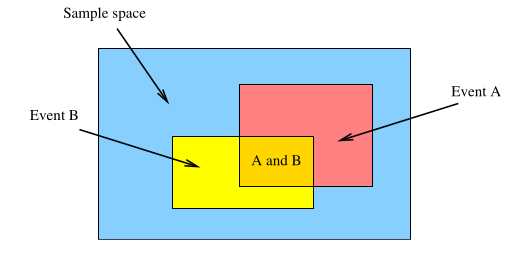
\includegraphics[width=5cm]{probs_ax.png}
\end{center}

\subsubsection{Derivied theorems}
\cor{Complement Rule
}{
    \[
        P(\lnot A) = 1- P(A)
    \]
}
\pf{Dm}{
\[
P(A \cup \neg A) = P(A) + P(\neg A) - P(A \cap \neg A)
\]

But: 
\[
P(A \cup \neg A) = P(\text{True}) = 1
\quad \text{and} \quad
P(A \cap \neg A) = P(\text{False}) = 0
\]

Therefore:
\[
1 = P(A) + P(\neg A) - 0
\quad \implies \quad
P(\neg A) = 1 - P(A) \qed
\]

}

\cor{Partition Rule}{
    \[
        P(A) = P(A \cap B) + P(A \cap \neg B)
    \]
}
\pf{Proof}{
    \[
\begin{aligned}
A &= A \cap (B \cup \neg B) &\text{[since $B \cup \neg B$ is always True]}\\
  &= (A \cap B) \cup (A \cap \neg B) &\text{[distributive law]}
\end{aligned}
\]

Hence,
\[
\begin{aligned}
P(A) &= P((A \cap B) \cup (A \cap \neg B)) \\
     &= P(A \cap B) + P(A \cap \neg B) - P((A \cap B) \cap (A \cap \neg B)) \\
     &= P(A \cap B) + P(A \cap \neg B) - P(\text{False}) \\
     &= P(A \cap B) + P(A \cap \neg B)
\end{aligned}
\]

}
\subsubsection{Multivalued Discrete Random Variables}
\dfn{
    k-value Discrete Random Variables
}{
    A random variable $A$ is \textit{$k$-valued discrete} if it takes exactly one value from 
    \[
    \{\nu_1, \nu_2, \dots, \nu_k\}.
    \]
}

\mprop{Key proprieties}{
    \begin{enumerate}
    \item \textbf{Mutual exclusivity:} For $i \neq j$,
    \[
        P(A = \nu_i \cap A = \nu_j) = 0
    \]

    \item \textbf{Exhaustiveness:}
    \[
        P(A = \nu_1 \cup A = \nu_2 \cup \dots \cup A = \nu_k) = 1
    \]
\end{enumerate}

}

\subsubsection{Conditional Probability}
\dfn{Conditional probs}{
    The Conditional probs of the event $A$ \textit{given} the event $B$ is defined as the quantity
    \begin{center}
        \begin{math}
            P(A\mid B) = \frac{P(A\cap B)}{P(B)}            
        \end{math}
    \end{center}
}

\cor{Cahin roule}{
    \[
        P(A\cap B) = P(B)P(A\mid  B)= P(A) P(B\mid A)
    \]
}
\subsubsection{Independent Events}
\dfn{Independent Events}{
    Events $A$ and $B$ are independent when:
    \begin{center}
        \begin{math}
            P(A\mid  B) = P(B)
        \end{math}
    \end{center}
}
(Meaning: B provides no information about A.)
\cor{consequences}{
    \begin{itemize}
        \item $P(A\cap b) = P(A)P(B)$ (from chail roule)
        \item $P(B|A) = P(B)$ (symmetry)
    \end{itemize}
}

\subsubsection{Bayes' Rule: The Heart of Probabilistic ML (ok chat... really?)}
\thm{Bayes's roule}{
    Now we have Bayes roule
    \begin{center}
        \begin{math}
            P(A\mid  B) = \frac{P(A)  P(B\mid A)}{P(B)}
        \end{math}
    \end{center}
}
\pf{Proof}{
    It's true by the chain roule that: $P(A \cap B) = P(B)  P(A\mid B)$. It's true also the reverse case $P(A \cap B) = P(B) · P(A\mid B)$.

    Since both expressions equal $P(A \mid B)$, they must equal each other:
    \[
        P(A)  P(B\mid A) = P(B)  P(A\mid B) 
    \]
    that it's equal to
    \[
        P(A\mid B) =\frac{[P(A)  P(B\mid A)]}{P(B)}
    \]
}
\ex{The trousers problem}{
    Setup:
    \begin{itemize}
        \item 60\% of students are boys, 40\% are girls
        \item girls wear in the same number skirt and trousers
        \item boys only wear trousers
    \end{itemize}
    If we see a student wearing trousers, what is the probability that is a girl?
}
\pf{Solution}{
    The probs a priori that a strudent is a girl is
    \[
        P(G) = \frac{2}{5}
    \]
    the probability that a student wears trousers is
    \[
        P(T) = \frac{1}{5} + \frac{3}{5} = \frac{4}{5}
    \]
    the probability that a student wear trousers, given that the student is a girl, is
    \[
        P(T\mid G) = 1/2
    \]
    So 
    \[
        P(G\mid T) =\frac{p(G)p(T\mid G)}{P(T)}=\frac{2/5\cdot 1/2}{4/5} = 1/4
    \]
}

\paragraph{Machine Learning Form}
\paragraph{Machine Learning Form}
For discrete $Y$ with values $\{y_1, y_2, \ldots, y_m\}$ and $X$ with values $\{x_1, x_2, \ldots, x_n\}$:
\[
P(Y = y_i \mid X = x_j) = \frac{P(Y = y_i) \cdot P(X = x_j \mid Y = y_i)}{P(X = x_j)}
\]

\textbf{Expanding the denominator:}
\begin{align*}
P(X = x_j) &= \sum_{i} P(X = x_j, Y = y_i) \quad \text{[sum over all $Y$ values]} \\
           &= \sum_{i} P(Y = y_i) \cdot P(X = x_j \mid Y = y_i) \quad \text{[chain rule]}
\end{align*}

\textbf{Complete Bayes' Rule:}
\[
P(Y = y_i \mid X = x_j) = \frac{P(Y = y_i) \cdot P(X = x_j \mid Y = y_i)}{\sum_{i} P(Y = y_i) \cdot P(X = x_j \mid Y = y_i)}
\]

\textbf{Terminology:}
\[
\underbrace{P(Y \mid X)}_{\text{posterior}} = \frac{\overbrace{P(X \mid Y)}^{\text{likelihood}} \cdot \overbrace{P(Y)}^{\text{prior}}}{\underbrace{P(X)}_{\text{marginal}}}
\]

\begin{itemize}
    \item \textbf{Posterior} $P(Y \mid X)$: What we want -- probability of $Y$ given observed $X$
    \item \textbf{Likelihood} $P(X \mid Y)$: How likely is $X$ if $Y$ is true?
    \item \textbf{Prior} $P(Y)$: What we believed before seeing $X$
    \item \textbf{Marginal} $P(X)$: Overall probability of observing $X$ (normalization constant)
\end{itemize}

\textbf{Alternative form:}
\[
\text{Posterior} = \frac{\text{Likelihood} \cdot \text{Prior}}{\text{Marginal Likelihood}}
\]
where:
\[
\text{Marginal} = \sum_{Y} P(X \mid Y) \cdot P(Y)
\]

The term ``marginal'' means we've \textbf{marginalized} (integrated/summed) over $Y$.

\section{The Joint Distribution}

\dfn{Joint Distribution}{
    Let $X_1, X_2,\dots, X_n$ be discrete random variables. The \textit{joint probability distribution} (or \textit{joint distribution}) of these variables is the function:
    \begin{center}
        \begin{math}
            P(X_1 = x_1, X_2 = x_2, \dots, X_n = x_n)
        \end{math}
    \end{center}

    which assigns to every possible combination of values \( (x_1, x_2, \dots, x_n) \) the probability that the random variables simultaneously take those values.

    Formally, for discrete variables, the joint distribution satisfies:
    \begin{itemize}
        \item \( 0 \leq P(x_1, x_2, \dots, x_n) \leq 1 \) for all \( (x_1, \dots, x_n) \)
        \item \( \sum_{x_1} \sum_{x_2} \cdots \sum_{x_n} P(x_1, x_2, \dots, x_n) = 1 \)
    \end{itemize}
}

Let's see an example
\ex{Joint distribution}{
    \begin{itemize}
        \item build a table with all possible combinations of values of random variables (features)
        \item compute the probability for any different combination of values
    \end{itemize}

    \begin{center}
        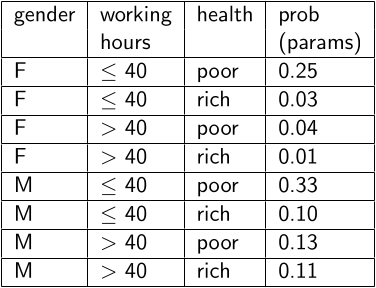
\includegraphics[width=6cm]{jd_img.png} % the table of the document
    \end{center}

    This table is the "Joint distribution"!

    Having that we may compute the probability of any event expressible as a logical combination of the features, with this formula
    \[
        P(E) = \sum_{row\in E} (row)
    \]
    in words for calculating an event we must add each row that is contained by the event. Let's provide an example (of an example)

        Let us compute the probability $P(M, poor)$
        \begin{center}
            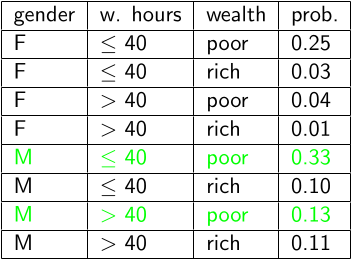
\includegraphics[width=6c]{jd_ex.png}
        \end{center}
    

    we have: $P(M, poor) = 0.33 + 0.13 = 0.46$
}

\subsection{Inference with the Joint distribution}
Here are with the inference:
\dfn{Contintional probability}{
    Let \( E_1 \) and \( E_2 \) be two events defined as logical conditions over subsets of the random variables (e.g., \( E_1: X_i = a, X_j = b \); \( E_2: Y = y \))

    Then, \textit{conditional probability} of \( E_1 \) given \( E_2 \) is:
    \[
        P(E_1 \mid E_2) = \frac{P(E_1 \land E_2)}{P(E_2)} = 
        \frac{\displaystyle\sum_{{row} \in (E_1 \land E_2)} P({row})}
        {\displaystyle\sum_{{row} \in (E_2)} P({row})}
    \]
}

for instance:
\ex{Conditional probability}{
    Let's compute $P(M|poor ) =\frac{P(M \land poor)}{P(poor)}$. We know that $P(M, poor ) = 0.46$. Let us compute $P(poor )$:
    \begin{center}
        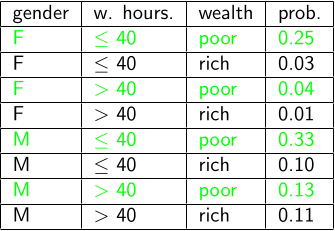
\includegraphics[width=6cm]{joint_inf.png}
    \end{center}
    Easy! $P(poor) = .75 \land P(M|poor) = 0.46/0.75 = 0.61$
}

\subsection{Complexity issues}
Let us build the joint table relative to
\[
    P(Y = wealth|X_1 = gender , X_2 = orelav.)
\]

\begin{center}
    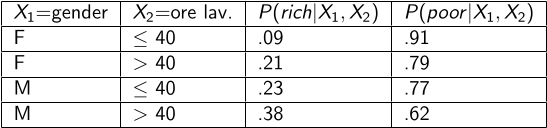
\includegraphics[width=6cm]{comp_issue.png}
\end{center}
To fill the table we need to compute $4=2^2$ parameters

If we have $n$ random variable $X = X_1 \times X_2 ,\dots, X_n$ where each $X_i$ is
boolean, we need to compute $2^n$ parameters. These parameters are \textit{probabilities}: to get reasonable value we would need a huge amount of data.

In particular the The Joint Distribution Requires \textit{Exponential parameters}
\ex{features and params}{
    \begin{itemize}
        \item With just 10 binary features, you need $2^{11}-1=2047$ parameters
        \item With 20 features: over 1 million parameters
        \item With 100 features: $2^{101}$ a number larger than the estimated atoms in the observable universe.
    \end{itemize}
}
This is computationally and statistically infeasible.
\subsubsection{USing Bayes}
for reducing complexity, we can rewrite the formula with the Bayes' rule:
\[
    P(Y=y_i\mid X=x_j) = \frac{P(Y=y_i)\cdot P(X = x_j\mid Y = y_i)}{\sum_i P(Y=y_i)\cdot P(X=x_j \mid Y=y_i)}
\]
generalising:
\[
    P(Y \mid X_1, X_2, \dots, X_n) = \frac{P(Y) \cdot P(X_1, X_2, \dots, X_n \mid Y)}{P(X_1, X_2, \dots, X_n)}
\]

But... there is a problem, it's required to know 
\[
    P(X_1, X_2, \dots, X_n \mid Y)
\]

that is the joint distribution of the features given $Y$, that requires, another time, $2^n$ params

\subsection{Naive Bayes}
For atteniung the complexity, it's possible assume an indipendencies conditional hypotesis, called "Naïve Bayes":
\[
    P(X_1,X_2,\dots,X_n|Y)=\prod_{i}P(X_i |Y)
\]
So given $Y$, $X_i$ and $X_j$ are independent from each other. In other therms:
\[
    P(X_i|X_j,Y)=P(X_i|Y)
\]
\nt{
    This means: onece we know $Y$, the feature $X_i \forall i$ are independents between each others
}
\ex{example 1}{
    A box contains two coins: a regular coin and a fake two-headed coin ($P(H) = 1$).Choose a coin at random, toss it twice and consider the following events:

    \begin{itemize}
        \item $A =$ First coin toss is H
        \item $B =$ Second coin toss is H
        \item $C =$ First coin is regular
    \end{itemize}
}
\ex{example 2}{
    For individuals, height and vocabulary are not independent, but they are if age is given.
}

\subsubsection{Giga formula with naive bayes}
\thm{Bayes rule}{
    \[
       P(Y = y_i \mid X_1, \dots, X_n) = \frac{P(Y = y_i) \cdot P(X_1, \dots, X_n \mid Y = y_i)}{P(X_1, \dots, X_n)}
    \]
}
\pf{Proof}{
    Left to mesco as exercice
}

\thm{Naïve Bayes}{
    \[
    P(Y = y_i \mid X_1, \dots, X_n) = \frac{P(Y = y_i) \cdot \prod_j P(X_j \mid Y = y_i)}{P(X_1, \dots, X_n)}
    \]
}
\pf{Proof}{
    Left to Bonzo as exercice
}

\thm{Classification of a new sample $x^{\text{new}} = \langle x_1, \dots, x_n \rangle$}{
    \label{thm:cne}
    Given a new instance represented by the feature vector $x^{\text{new}} = (x_1, x_2, \dots, x_n)$, 
    the predicted class is obtained as:
    \[
        Y^{\text{new}} = \arg\max_{y_i} \, P(Y = y_i) \cdot \prod_{j} P(X_j = x_j \mid Y = y_i)
    \]
}

\pf{Proof}{
    Left to Bastiality as an exercise.
}

\nt{
    Theorem~\ref{thm:cne} expresses the decision rule of the Naïve Bayes classifier.
    Given a new vector of features $x^{\text{new}} = (x_1, x_2, \dots, x_n)$, 
    we estimate the most probable class $y_i$ by maximizing the posterior probability 
    $P(Y = y_i \mid X_1 = x_1, \dots, X_n = x_n)$, 
    which—under the conditional independence assumption—reduces to the product of the prior $P(Y = y_i)$ 
    and the individual likelihoods $P(X_j = x_j \mid Y = y_i)$.
}




\end{document}
